

% Note that the a4paper option is mainly intended so that authors in
% countries using A4 can easily print to A4 and see how their papers will
% look in print. Authors are encouraged to use U.S. letter paper when 
% submitting to IEEE. Use the testflow package mentioned above to verify
% correct handling of both paper sizes by the author's LaTeX system.
%
% Also note that the "draftcls" or "draftclsnofoot", not "draft", option
% should be used if it is desired that the figures are to be displayed in
% draft mode.
%
% This paper can be formatted using the peerreviewca
% (instead of conference) mode.
\documentclass[conference]{IEEEtran}
\usepackage{graphicx}
\graphicspath{ {./figures/} }
\usepackage{amsmath,amssymb}
\interdisplaylinepenalty=2500
\usepackage[ruled,vlined]{algorithm2e}
\usepackage[english]{babel}
\usepackage{lipsum}  
\usepackage{hyperref}
\usepackage{cite}  
\usepackage{siunitx}
\usepackage{booktabs}
\sisetup{separate-uncertainty}

% correct bad hyphenation here
\hyphenation{op-tical net-works semi-conduc-tor IEEEtran}


\begin{document}

% paper title
\title{Assessment of Multi-Modal Reward Functions in Reinforcement Learning for Urban Traffic Control under Real-World limitations}


% author names and affiliations
% use a multiple column layout for up to three different
% affiliations
\author{\authorblockN{Alvaro Cabrejas Egea}
\authorblockA{MathSys Centre for Doctoral Training,\\
University of Warwick \& Vivacity Labs, London, UK\\
Email: a.cabrejas-egea@warwick.ac.uk}
\and
\authorblockN{Colm Connaughton}
\authorblockA{Warwick Mathematics Institute\\
University of Warwick\\
Email: c.p.connaughton@warwick.ac.uk}
}


\maketitle

\begin{abstract}
The abstract goes here.
\end{abstract}



\IEEEpeerreviewmaketitle



\section{Introduction}
%\lipsum(1)

\section{Related Work}
%\lipsum()

As indicated in \cite{survey2020}, pedestrian implementation has a high impact on learning performance, being often discarded as unimportant or left for future work.

In this paper we attempt to cover this gap in the literature, providing with a performance assessment of RL agents serving both vehicles and pedestrians, using a variety of rewards in a calibrated model of a real-world junction.
\section{Problem Definition}
\subsection{Markov Decision Processes and Reinforcement Learning}
The problem is framed as a Markov Decision Process (MDP), satisfying the Markov property: given a current state $s_t$, the next state $s_{t+1}$ is independent of the succession of previous states $\{s_{t-1}, s_{t-2}, ..., s_0\}$.
An MDP is defined by the 5-element tuple:
\begin{enumerate}
\item The set of possible states $\mathcal{S}, s_i\in \mathcal{S}$.
\item The set of possible actions $\mathcal{A}, a_i\in \mathcal{A}$.
\item The probabilistic transition function between states $\mathcal{T}$.
\item The discount factor $\gamma \in [0,1]$ 
\item The scalar Reward Function $\mathcal{R}$. 
\end{enumerate}

The objective of an MDP agent is to find an optimal policy $\pi^*$, mapping states to actions, that maximises the sum of expected discounted reward.
\begin{equation}
R_t = \mathbb{E} \bigg{[} \sum^{\infty}_{i=0} \gamma^i r_{t+i} \bigg{]} 
\label{eq:reward}
\end{equation}
In this case, $\mathcal{T}$ is unknown, only allowing for model-free Reinforcement Learning (RL).

Model-Free RL is an area of Machine Learning covering how independent agents can take sequential decisions in an unknown environment and learn from these in order to obtain $\pi^*$. 
There are two main approaches: Policy-Based RL, in which states are mapped to a distribution of potential actions, and Value-Based RL, which is used in this paper and estimates the value (expected return) of the different state-action pairs under a given policy $\pi$ as defined in Eq. \ref{eq:value}.
\begin{equation}
V^{\pi}(s) = \mathbb{E} [R_t|s,\pi]
\label{eq:value}
\end{equation}

\subsection{Q Learning and Value-Based RL}
Q-Learning\cite{watkins} is an off-policy value-based RL algorithm. For any finite MDP, it can find an optimal policy (maximise expected total discounted reward) starting from the current state\cite{melo}.
Q-Learning aims to learn an optimal action-value function $Q^*(s,a)$, defined as the total return after being in state $s$, taking action $a$ and then following policy $\pi^*$. %as shown in Eq.\ref{eq:qlearning}.
\begin{equation}
Q^*(s,a) = \max_{\pi} \mathbb{E} \big[ R_t | s=s_t, a=a_t, \pi^* \big]
\label{eq:qlearning}
\end{equation}
Traditional table-based Q-Learning approximates $Q^*(s,a)$ recursively through successive Bellman updates,
\begin{equation}
Q^{\pi}(s_t,a_t) \leftarrow Q^{\pi}(s_t,a_t) + \alpha \big( y_t - Q(s_{t+1},a) \big)
\label{eq:bellmanupdate}
\end{equation}
with $y_t$ being the Temporal Difference(TD) target for the Q-function.
\begin{equation}
y_t = R_t + \gamma \,\,\, \max_{a_{t+1}} Q^{\pi}(s_{t+1},a_{t+1})
\end{equation}

This table representation is not useful for high dimensionality cases, since the size of our table would increase exponentially, nor for continuous cases, since every distinct $s\in\mathcal{S}$ would require an entry.

\begin{figure}                                                
\centering                                                    
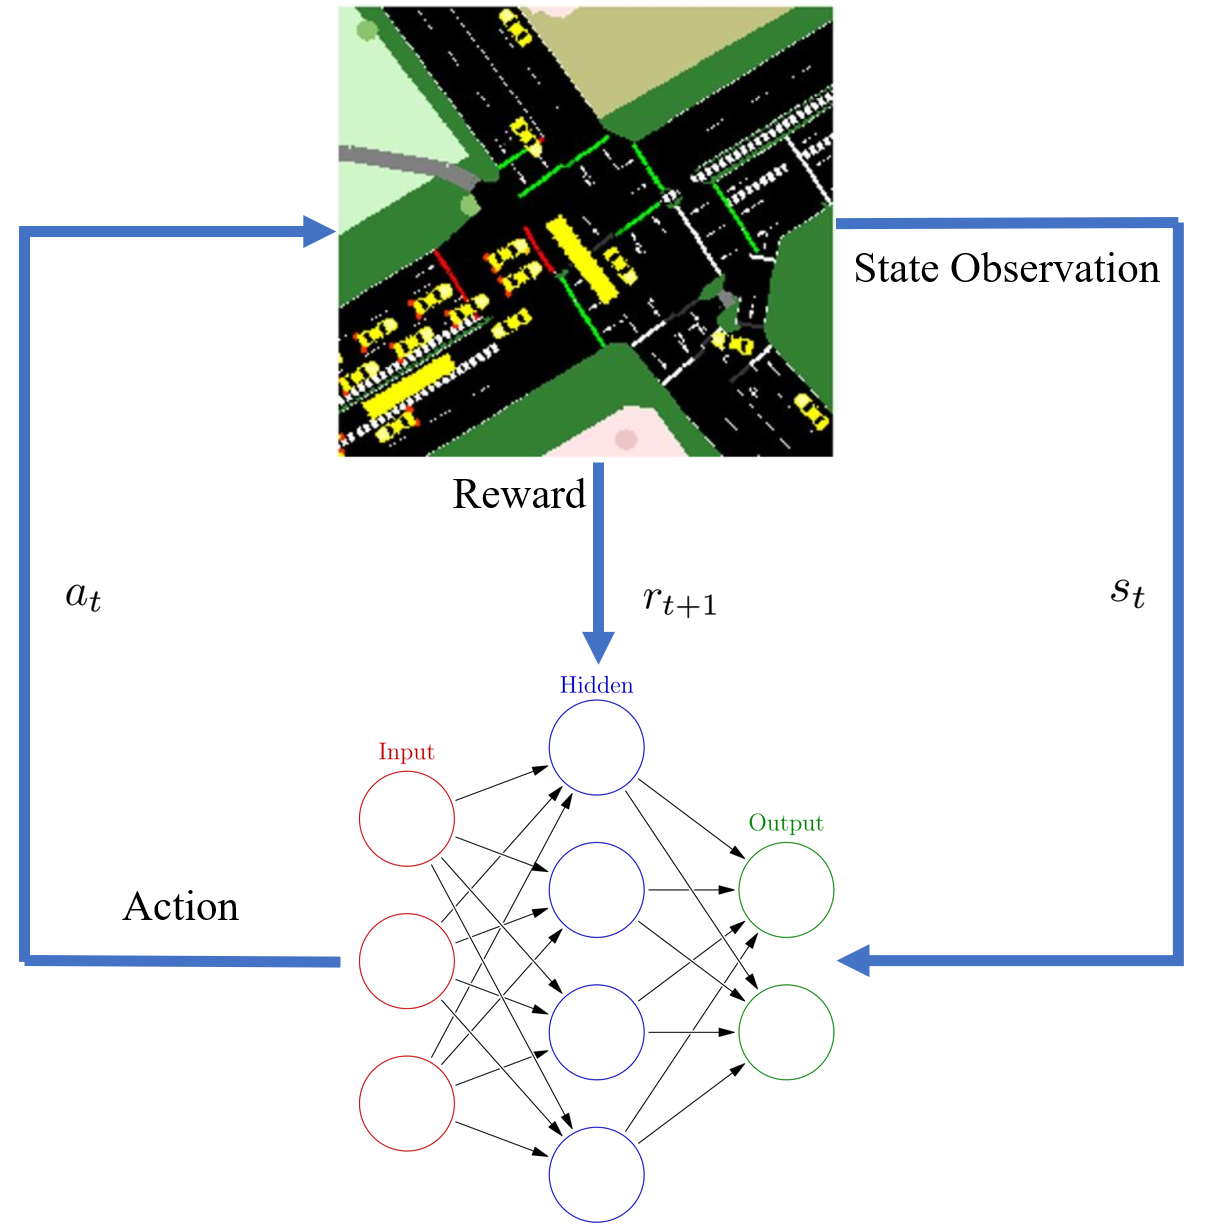
\includegraphics[width=2.5in]{schematic_pp2.png}                                    
\caption{Schematic representation of information transmission in Reinforcement Learning taking place between Agent and SUMO Environment}                                  
\label{rl}                                               
\end{figure}  

\subsection{Deep Q Network}
One way of dealing with the issues of Q-Learning in high dimensional spaces is to use a Neural Network as function approximator, called Deep Q-Network (DQN) \cite{mnih2015}.
The Q-function approximation is denoted then in terms of the parameters $\theta$ of the DQN as $Q(s,a,\theta)$.
One component of DQN that stabilises learning is the Target Network. DQN uses two neural networks: the main network with parameters $\theta$, which approximates the Q-function, and the target network with parameters $\theta^-$ which provides the TD targets for the DQN updates and is updated every number of episodes by copying the weights $\theta^- \leftarrow \theta$. With $Q^{\pi} (s_{t+1}, a_{t+1}, \theta^-)$ representing the target network, it results in a TD target to approximate:
\begin{equation}
y_t = R_t + \gamma \,\,\, \max_{a_{t+1}} Q^{\pi} (s_{t+1}, a_{t+1}, \theta^-)
\end{equation}
\section{Methods}
\subsection{Reinforcement Learning Agent}
The basic common agent used to obtain these results is a standard implementation of a DQN in PyTorch \cite{pytorch}, optimising its weights via Stochastic Gradient Descent \cite{kiefer} using ADAM \cite{adam} as optimizer.
The learning rate is $\alpha=10^{-5}$ and the discount factor is $\gamma = 0.8$ for all simulations.
The Neural Network in the agent uses 2 hidden, fully connected layers of sizes 500 and 1000 respectively, using ReLU as an activation function.
\subsection{Reinforcement Learning Environment}
The environment is modelled in the microscopic traffic simulator SUMO \cite{sumo}, representing a real-world intersection in Greater Manchester, UK.
The junction consists of four arms, with 6 incoming lanes (two each in North-South orientation, and one each in East-West orientation) and 4 pedestrian crossings.
The real-world site also contains 4 Vivacity vision-based sensors, able to supply queue length, speed and flow data.
The demand and turning rations at the junction have been calibrated using 3.5 months of journey time and flow data collected by these sensors.
The environment includes an emulated traffic signal controller, responsible of changing between the different stages in the intersection and enforcing the operational limitations, focused on safety.
This includes enforcing green times, intergreen times, as well as determining allowed stages.  

A stage is defined as a group of non-conflicting green lights (phases) in a junction which move at the same time.

The Agent decides which stage to select next and requests this from an emulated traffic signal controller, which moves to that stage subject to its limitations, which are primarily safety-related.
The site features 4 Vivacity vision-based sensors which can provide flow, queue length and speed data. The data available to the agent is restricted to what can be obtained from these sensors.
\begin{figure}                                                
\centering                                                    
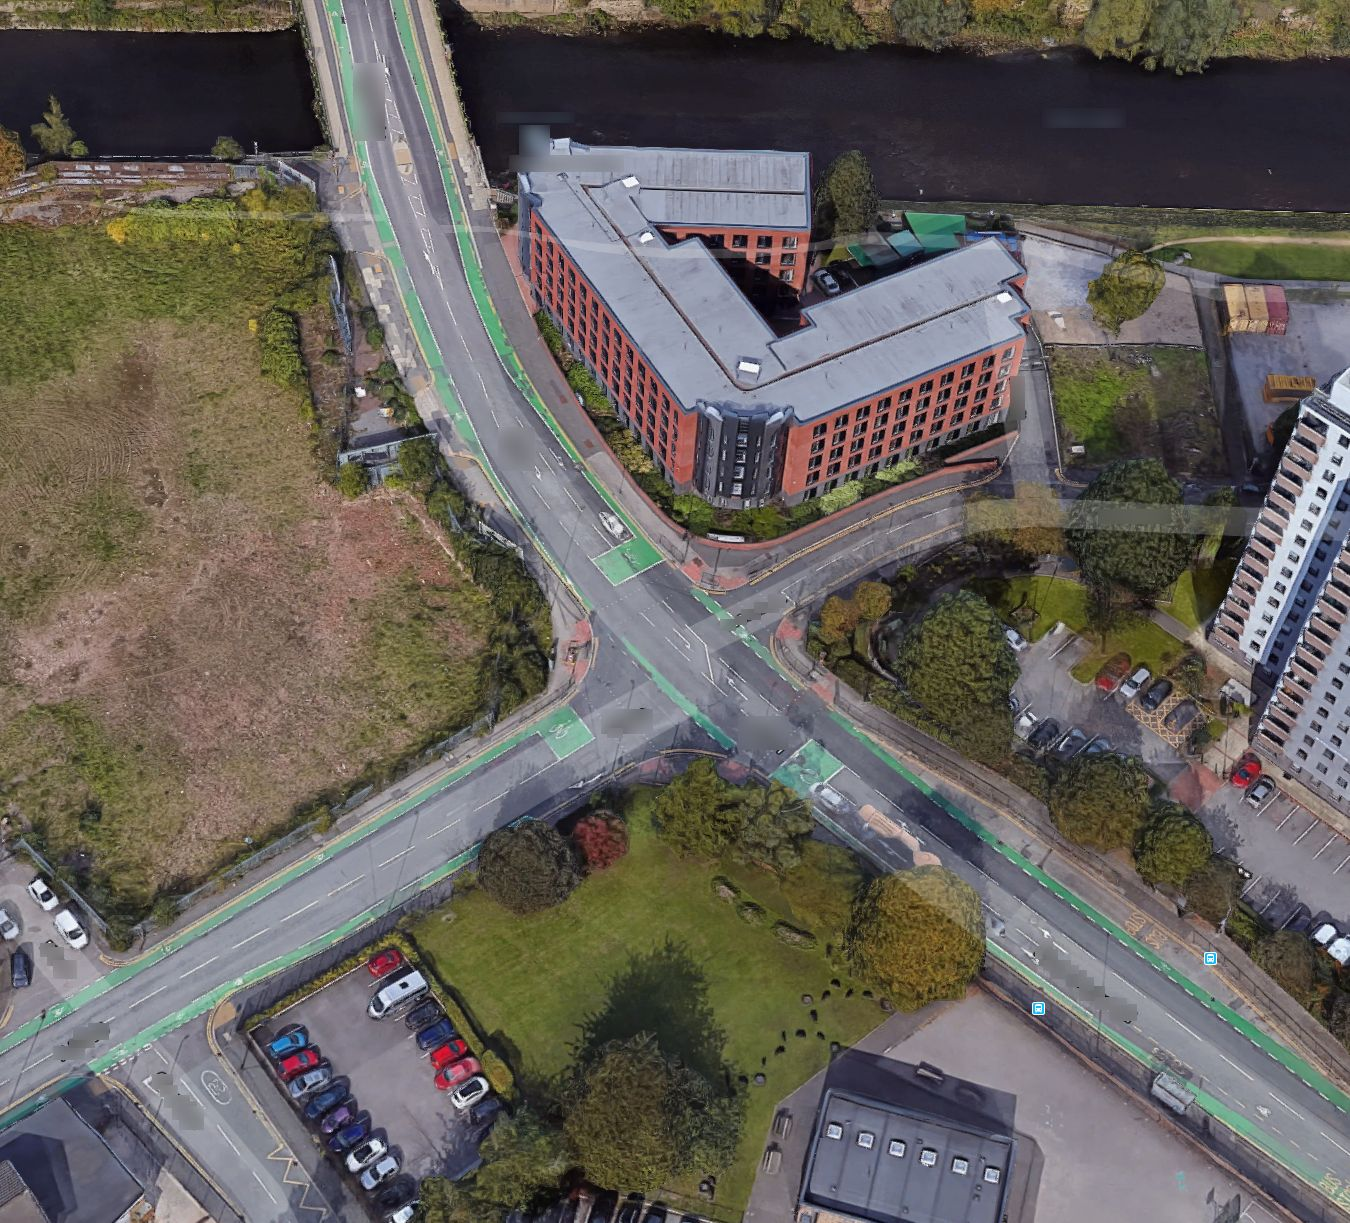
\includegraphics[width=2.5in]{gmaps_iso_censored.jpg}                                    
\caption{Aerial view of Study Junction from Google Earth.}                                  
\label{intersection}                                               
\end{figure}     

\begin{figure}                                                
\centering                                                    
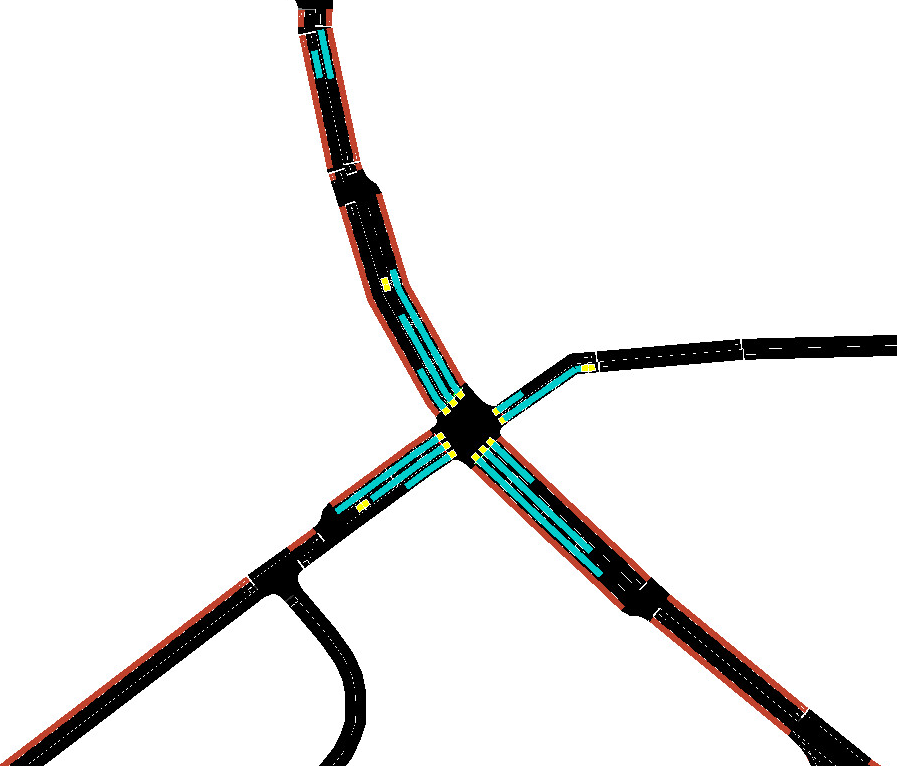
\includegraphics[width=2.5in]{intersection}                                    
\caption{Study Junction model in SUMO with a schematic representation of the areas covered by sensors.}                                  
\label{intersection}                                               
\end{figure}     

\subsection{State Representation}
The agent receives an observation of the simulator state as input, which remains constant across all experiments here presented.
This observation is a combination of the state of the traffic controller (which stage is active) and data from the sensors.
The data from the sensors is comprised of the occupancy in each lane area detector and a binary signal representing whether the "Pedestrian Cross" button has been pushed or not.
A series of these, covering the last 12 seconds at a resolution of 0.6 seconds (20 state-entries) are provided to the agent.

While there is a variety of state representations available in the literature, often being more information dense, many of their features are not obtainable in practice with available sensors.
Furthermore, recent studies \cite{genders2018} show that more information-dense states provide marginal improvements, if any, being able to control isolated intersections with simple inputs.

\begin{itemize}
\item 7 * Area sensor occupancies
\item VDR3 Pedestrian Button Push
\item G1-G4 Stage bits (Binary, active/inactive)
\item NS1-NS4 Next Stage Bits (ASK SHAUN WHERE THEY COME FROM, FUNCTION AND HOW TO OBTAIN THEM)
\end{itemize}

\subsection{Actions of the Agent}
The actions available to the agent

The junction is configured to have 4 available stages. 
The Agent is able to choose Stage 2, Stage 3 or Stage 4, yielding an action space size of 3.
Stage 1 serves a leading right turn phase from the main road, and was excluded by suggestion of the transport authority, since it is an intermediary stage that the controller will go through in order to reach Stage 2, which serves the main road.
Stage 3 only serves pedestrians, which are not considered here, so was also excluded.
Stage 4 serves the side roads, which do experience significant demand.
In each timestep when a stage has been active longer than the minimum green time, the agent generates state-action values for each potential stage and the highest value is chosen according to an $\epsilon$-greedy policy \cite{suttonbarto}. If the agent chooses the same stage, that stage is extended by 0.6s, otherwise the controler begins the transition to the other stage.
The extension can be chosen indefinitely, as long as the agent identifies it as the best action.

The complexity in the decision-making stems from the combination of using of Stage 1 as an intermediate state and the extensions to the stage duration.
Traditional RL for Urban Traffic Control regards each Stage as an action for the agent to take, based on the instantaneous state of the system.
However, in the case of the intermediate Stage 1, the agent has to choose when to start the transition without knowledge of the future state when Stage 2 begins.
Regarding the extensions, given that their length is smaller than that of the initial phase, their impact on the state will be smaller, generating a distribution of reward and state-action value outcomes that the agent needs to approximate.
\begin{figure}                                                
\centering                                                    
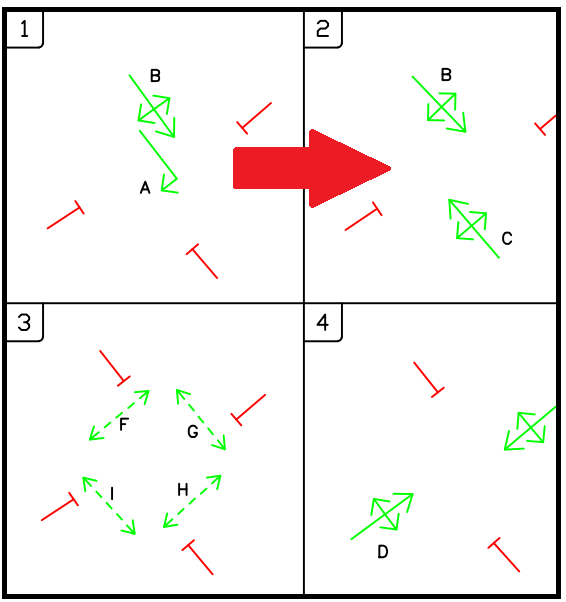
\includegraphics[width=2.5in]{phases_limited.png}                                    
\caption{Allowed stages and the phases that compose them. Stage 1 is an intermediate Stage, being necessary to go through it to reach Stage 2.}                                  
\label{intersection}                                               
\end{figure}     

\subsection{Modal Prioritisation}
The agent has to serve vehicles and pedestrians arriving at the intersection, seeking to jointly optimise the intersection for both modes of transport.

All the reward functions presented in this paper follow the same structure.
The reward, as seen by the agent, will be a linear combination of an independently calculated reward for the vehicles and another for the agents, as it can be seen in Eq. \ref{eq:modal}.
\begin{equation}
R_t = \alpha * R^v_t + \beta * R^p_t
\label{eq:modal}
\end{equation}
In this way, $\alpha$ and $\beta$ are the Modal Prioritisation coefficients for our rewards.

\section{Reward Functions}
\section{Results}
\begin{figure*}                                                
\centering                                                    
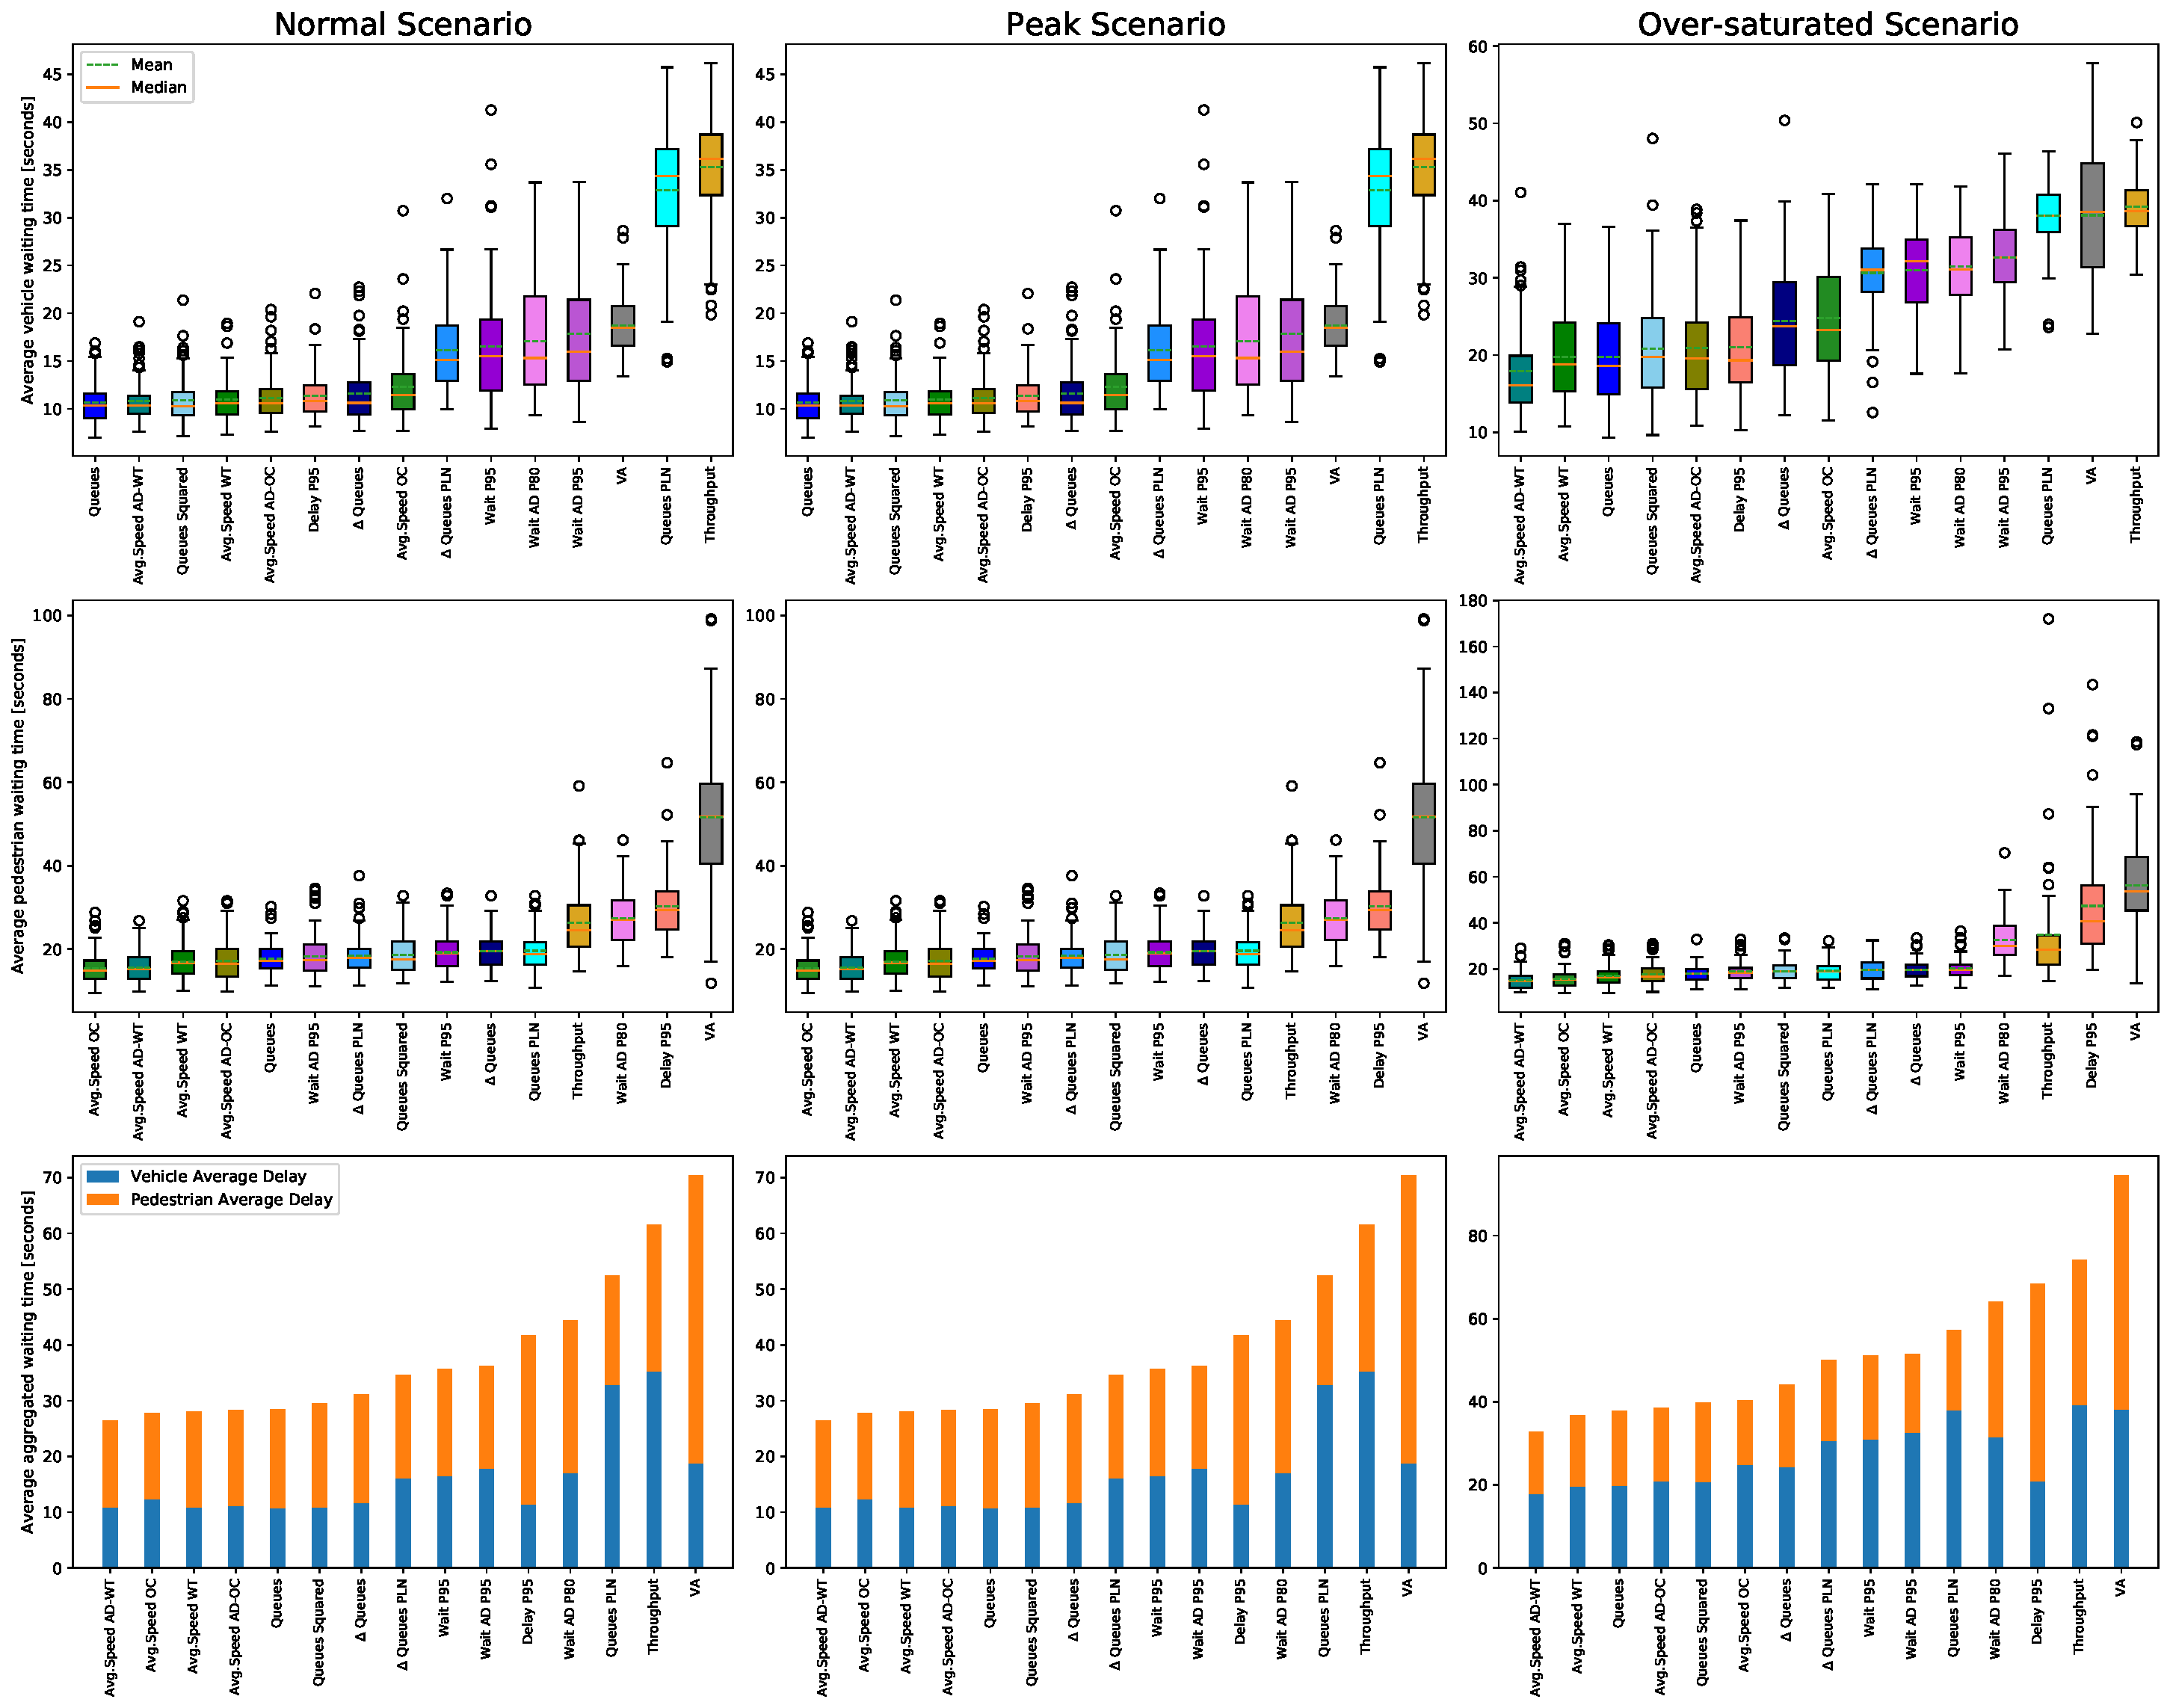
\includegraphics[width=\textwidth]{9grid_ordered_boxplot_all.pdf}                                    
\caption{Average waiting time for the best performing agents across all three demand scenarios.}                                  
\label{results_9_grid}                                               
\end{figure*}
\section{Discussion and Conclusion}

In this section the individually tested reward functions are introduced.

Let $N$ be the set of lane queue sensors present in the intersection.
Let $M$ be the set of pedestrian occupancy sensors in the junction.
Let $V_t$ and $P_t$ be respectively the set of vehicles on incoming lanes, and the set of pedestrians waiting to cross in the intersection at time $t$. 
Let $s_v$ be the individual speeds of the vehicles, $\tau^v$ and $\tau^p$ the waiting times of vehicles and pedestrians respectively.
Let $\rho_v$ and $\rho_p$ the vehicular and pedestrian flows across the junction over the length of the action.
Let $t^p$ be the time at which the previous action was taken and $t^{pp}$ the time of the action before that.
Lastly, let $t^v_e$ and $t^p_e$ be the entry times of vehicles and pedestrians to the area covered by sensors. 

\subsection{Queue Length based Rewards}
\subsubsection{Queue Length}
The reward will be the negative sum over all $n$ sensors of the queues ($q$) at time step $t$.
Similar to the reward introduced in \cite{prashanth2011} but without the need for thresholding the queue values, and used in \cite{aslani2019}.
\begin{equation}
    R_t = - \alpha \sum_{n \in N} q^v_{t} - \beta \sum_{m \in M} q^p_{t}
\label{eq:queue}
\end{equation}
One of the first published in the field of Q-Learning, this reward function has low sensor requirements and is implementable using just induction loops.

\subsubsection{Queue Squared}
Introduced in \cite{gendersthesis}, this function squares the result of adding all queues.
This increasingly penalises actions that lead to longer queues.
\begin{equation}
   R_t = - \alpha \bigg( \sum_{n \in N} q^v_{t} \bigg)^2 - \beta \bigg( \sum_{m \in M} q^p_{t} \bigg)^2
\label{eq:queuesq} 
\end{equation}

\subsubsection{Delta Queue}
The reward will be the difference between the previous and current sum of queues, turning positive for those action that decrease the queue size and negative when it increases.
Similar approach to the rewards shown in Eqs. (\ref{eq:delta_wait_time}) and (\ref{eq:changedelay}).
\begin{equation}
    R_t = \alpha \bigg( \sum_{n \in N} q^v_{t^p} -\sum_{n \in N} q^v_{t} \bigg) + \beta \bigg( \sum_{m \in M} q^p_{t^p} - \sum_{m \in M} q^p_{t} \bigg)
    \label{deltaqueue}
\end{equation}

\subsection{Waiting Time based Rewards}
\subsubsection{Wait Time}
The reward will be the negative aggregated time in queue ($\tau$) that the vehicles at the intersection have accumulated since the last action. 
\begin{equation}
R_t = - \bigg( \sum_{v \in V_t} \tau^v_{t} + \sum_{p \in P_t} \tau^p_{t} \bigg)
\label{eq:wait_time}
\end{equation}
This function is more information-dense than queues, scaling with individual waiting times, but requires more advanced hardware for individual vehicle recognition.

\subsubsection{Delta Wait Time}
Similar to Eq. \ref{deltaqueue}, used in \cite{liang2018}. The reward will be the difference between total intersection $\tau$ between the current time and the previous action. 
\begin{equation}
R_t = \alpha \bigg( \sum_{v \in V_t} \tau^v_{t_p} -  \sum_{v \in V_t} \tau^v_{t} \bigg) + \beta \bigg( \sum_{p \in P_t} \tau^p_{t_p} -  \sum_{p \in P_t} \tau^p_{t} \bigg)
\label{eq:delta_wait_time}
\end{equation}

\subsubsection{Waiting Time Adjusted by Demand}
The reward will be the negative aggregated waiting time as above, but in this case it is divided by an estimate of the current demand ($\hat{d}$) or arrival rate, implicitly accepting that given a wait time as a result of an action, the penalty should scale with the difficulty of the task.
\begin{equation}
   R_t = -\frac{1}{\hat{d}} \bigg( \alpha \sum_{v \in V_t} \tau^v_{t} + \beta \sum_{p \in P_t} \tau^p_{t} \bigg)
\label{eq:wait_time_norm} 
\end{equation}

\subsection{Time Lost based Rewards}
\subsubsection{Time Lost}
Used in \cite{wan2018}, the reward will be the negative aggregated delay accumulated by all vehicles upstream from the intersection, understanding the delay as deviations from the vehicle's maximum allowed speed ($s_{max}$). 
Assuming a simulator time step of length $\delta$:
\begin{equation}
    R_t = - \bigg( \alpha \sum_{v \in V_t}  \sum_{t^p_e}^t \delta * \big( 1-\frac{s_v}{s_{max}} \big) + \beta \sum_{p \in P_t} \tau^p_t \bigg)
\label{eq:delay}
\end{equation}
This reward provides a more accurate representation of the total delay caused, since it also accounts for all deceleration happening around the intersection. 

\subsubsection{Delta Time Lost}
Introduced in \cite{abdulhai2010} and used in \cite{mannion} \cite{genders2016} \cite{gao2017} \cite{mousavi2017} and \cite{genders2018}.
Similar to Eq. (\ref{eq:delta_wait_time}).
The reward will be the change of global delay in the vehicles around the intersection since the last action was taken.
\begin{equation}
\begin{split}
R_t =  \alpha \bigg( \sum_{v \in V_t} \sum_{t^{pp}}^{t^p} ts * & \big( 1-\frac{s_v}{s_{max}} \big) - \sum_{v \in V_t}  \sum_{t^p}^t ts * \big( 1-\frac{s_v}{s_{max}} \big) \bigg) \\
& + \beta \bigg( \sum_{p \in P_t} \tau^p_{t^p} - \sum_{p \in P_t} \tau^p_{t} \bigg) 
\end{split}
\label{eq:changedelay} 
\end{equation}
This reward function provides both punishment and reward centered around zero.

\subsubsection{Delay Adjusted by Demand}
The reward will be the same as in the point above, but divided by an estimate of the demand level.
\begin{equation}
    R_t = -\frac{1}{\hat{d}} \bigg( \alpha \sum_{v\in V_t}  \sum_{t^p}^t ts * \big( 1-\frac{s_v}{s_{max}} \big) + \beta \sum_{p \in P_t} \tau^p_{t} \bigg)
\label{eq:delay}
\end{equation}

\subsection{Average Speed based Rewards}
\subsubsection{Average Speed, Wait Time Variant}
This reward seeks to maximise the average joint speed of all vehicles around an area of influence around the intersection. Let $\tau_{max}$ be a maximum desirable pedestrian waiting time.
\begin{equation}
    R_t = \alpha \frac{\sum_{v \in V_t} \frac{s}{s_{max}}}{\sum_{V_t} v}  + \beta \sum_{p \in P_t} \frac{\tau^p_{t}}{\tau_{max}}
\label{eq:avgspeed_wait}
\end{equation}

\subsubsection{Average Speed, Occupancy Variant}
This reward seeks to maximise the average joint speed of all vehicles around an area of influence around the intersection. Let $p_{max}$ be a maximum desirable number of pedestrians in the crossing.
\begin{equation}
    R_t =   \alpha \frac{ \sum_{v \in V_t} \frac{s}{s_{max}}}{\sum_{V_t} v} + \beta \sum_{p \in P_t} \frac{p}{p_{max}}
\label{eq:avgspeed_occ}
\end{equation}

\subsubsection{Average Speed Scaled by Demand, Demand and Occupancy}
The reward will be, as in the previous two entries, but multiplied by an estimation of the demand $\hat{d}$. This function scales the reward with the difficulty of the task.

\subsection{Throughput based Rewards}
\subsubsection{Throughput}
The reward will be the total number of vehicles that cleared the intersection between the last time that an action was taken and now.
\begin{equation}
    r_t = \alpha \sum_{t_p}^t \rho_v + \beta \sum_{t_p}^t \rho_p
\label{eq:throughput}
\end{equation}


\section{Experiments}

\subsection{DQN Agents Training}
The training process covered 1500 episodes running for 3000 steps of length $\delta=0.6$ seconds for a simulated time of 30 minutes (1800 seconds).
The traffic demand is increased as the training advances, with the agent progressively facing sub-saturated, near-saturated and over-saturated scenarios, with a minimum of 1 vehicle/3 seconds (1200 vehicles/h) and a maximum of 1 vehicle/1.4 seconds (2571 vehicles/h).

For each reward function, 10 copies of the agent were trained, and their performance was compared against two reference systems. These were Maximum Occupancy (longest queue first) and Vehicle Actuated System D \cite{highways}, commonly used in the UK. The agent performing best in each class was selected for scoring.
\subsection{Evaluation and Scoring}
Each agent is tested and its performance scored over 100 copies of 3 different scenarios with different demand levels. Each evaluation has the same length as the training episodes, and the demand is kept constant during each run.
These 3 scenarios are aimed to test the agents during normal operation, peak times and over-saturated conditions, and will be henceforth referred to as Normal, Peak and OverSat.
Peak Scenario uses the level of demand observed in the junction that results in saturated traffic conditions under traditional controllers.

The Normal Scenario uses an arrival rate of 1 vehicle / 2.1 seconds (1714 vehicles/h). Peak Scenario uses an arrival rate of 1 vehicle / 1.7 seconds (2117 vehicles/h). OverSat Scenario uses an arrival rate of 1 vehicle / 1.4 seconds (2400 vehicles/h)

Methods based on maximisation of the average speed seem to be Pareto Optimal in this context.
In them, the travel times are allocated in a way, such that attempting to optimise any of our result variables (i.e. vehicle travel time and pedestrian travel time) will have a negative impact on the other one.


\begin{table*}[!htp]
\centering
\setlength\tabcolsep{0pt}

\caption{Average waiting time in seconds for all agents across demand levels}
\label{tab:some example table}

\begin{tabular*}{\textwidth}{
  @{\extracolsep{\fill}}
  l
  S[table-format=-1.2(1)]
  S[table-format=-1.2(1)] 
  S[table-format=-1.2(1)]
  S[table-format=-1.2(1)]
  S[table-format=-1.2(1)]
  S[table-format=-1.2(1)]
  @{}
}
\toprule
& \multicolumn{2}{c}{Normal Scenario} &
\multicolumn{2}{c}{Peak Scenario} &
\multicolumn{2}{c}{Oversaturated Scenario} \\

Scenario & {Vehicles} & {Pedestrians} & {Vehicles} & {Pedestrians}  & {Vehicles}  & {Pedestrians}\\
\midrule
Queues                 & 7.87\pm 0.83 & 16.47\pm 3.95 & 10.68\pm 2.06 & 17.73\pm 3.64 & 19.80\pm 6.01 & 17.94\pm 3.48  \\
Queues Sq.             & 7.79\pm 0.93 & 18.55\pm 4.47 & 10.92\pm 2.41 & 18.60\pm 4.81 & 20.80\pm 6.88 & 19.02\pm 4.38  \\
Queues PLN             & 14.57\pm 4.91 & 20.31\pm 4.94 & 32.90\pm 6.36 & 19.59\pm 4.78 & 38.04\pm 3.93 & 19.28\pm 4.87  \\
$\Delta$ Queues        &  8.34\pm 1.04 & 18.37\pm 3.94 & 11.63\pm 3.09 & 19.45\pm 3.75 & 24.40\pm 7.20 & 19.70\pm 3.80  \\
$\Delta$ Queues PLN    & 10.37\pm 1.10 & 17.45\pm 3.59 & 16.11\pm 4.38 & 18.44\pm 4.45 & 30.64\pm 5.00 & 19.49\pm 4.32  \\
\midrule
Wait Time              & 7.80\pm 0.90 & 41.05\pm 19.40 & 14.65\pm 4.73 & 110.34\pm 59.56 & 28.82\pm 4.83 & 228.46\pm 159.81  \\
Wait Time AD           & 7.83\pm 0.99 & 56.00\pm 30.22 & 14.84\pm 4.84 & 169.11\pm 92.44 & 27.52\pm 5.01 & 324.12\pm 212.37  \\
$\Delta$ Wait Time     & 9.12\pm 1.23 & 82.57\pm 36.55 & 15.28\pm 5.09 & 326.07\pm 175.84 & 24.16\pm 6.77 & 594.03\pm 273.64  \\
\midrule
Wait Time P80          & 8.20\pm 1.26 & 28.80\pm 9.05 & 14.94\pm 4.81 & 54.29\pm 35.00 & 30.01\pm 4.84 & 113.68\pm 52.00  \\
Wait Time AD P80       & 8.25\pm 1.13 & 23.52\pm 5.73 & 17.05\pm 5.91 & 27.35\pm 6.29 & 31.43\pm 4.95 & 32.69\pm 9.67  \\
$\Delta$ Wait Time P80 & 8.94\pm 1.38 & 33.35\pm 17.34 & 16.68\pm 4.65 & 81.64\pm 49.48 & 30.38\pm 4.50 & 149.79\pm 105.07  \\
\midrule
Wait Time P95          & 8.26\pm 1.15 & 19.00\pm 4.67 & 16.51\pm 5.94 & 19.24\pm 4.44 & 31.02\pm 5.26 & 20.14\pm 4.16  \\
Wait Time AD P95       & 8.48\pm 1.19 & 18.07\pm 4.75 & 17.88\pm 6.25 & 18.30\pm 5.02 & 32.67\pm 5.28 & 18.78\pm 4.37  \\
$\Delta$ Wait Time P95 & 10.02\pm 1.66 & 42.36\pm 16.59 & 16.27\pm 5.33 & 72.27\pm 44.89 & 26.88\pm 6.22 & 174.85\pm 109.01  \\
\midrule
Delay                  & 6.39\pm 0.40 & 849.52\pm 318.33 & 8.59\pm 0.89 & 849.52\pm 318.33 & 14.43\pm 3.16 & 849.52\pm 318.33  \\
Delay AD               & 6.71\pm 0.43 & 811.38\pm 352.38 & 8.79\pm 0.96 & 811.38\pm 352.38 & 14.08\pm 3.31 & 811.38\pm 352.38  \\
$\Delta$ Delay         & 11.18\pm 2.93 & 211.41\pm 116.86 & 26.98\pm 6.75 & 546.51\pm 263.71 & 34.97\pm 3.45 & 393.81\pm 267.95  \\
\midrule
Delay P80              & 8.39\pm 1.10 & 46.78\pm 16.52 & 11.52\pm 2.36 & 78.91\pm 35.73 & 20.93\pm 7.02 & 143.27\pm 72.39  \\
Delay AD P80           & 7.74\pm 0.81 & 44.55\pm 17.51 & 10.68\pm 1.95 & 122.05\pm 112.18 & 18.92\pm 6.46 & 404.54\pm 252.47  \\
$\Delta$ Delay P80     & 10.62\pm 2.34 & 66.46\pm 30.32 & 20.51\pm 6.04 & 180.64\pm 107.80 & 29.70\pm 4.97 & 307.76\pm 218.11  \\
\midrule
Delay P95              & 7.92\pm 0.89 & 26.21\pm 4.86 &  11.38\pm 2.42 & 30.30\pm 7.64 & 20.99\pm 6.29 & 47.34\pm 23.27  \\
Delay AD P95           & 7.83\pm 0.84 & 48.76\pm 24.28 & 11.62\pm 3.02 & 180.59\pm 123.18 & 21.77\pm 6.82 & 425.35\pm 234.33  \\
$\Delta$ Delay P95     & 8.23\pm 1.29 & 99.40\pm 59.76 & 15.22\pm 4.97 & 221.92\pm 133.24 & 25.35\pm 6.43 & 398.13\pm 240.03  \\
\midrule
Throughput             & 18.71\pm 4.79 & 23.60\pm 6.88 & 35.28\pm 5.60 & 26.26\pm 8.14 & 39.24\pm 3.72 & 34.86\pm 28.54  \\
Throughput P80         & 35.53\pm 10.87 & 51.96\pm 31.20 & 47.60\pm 5.99 & 65.91\pm 37.86 & 47.85\pm 5.15 & 84.93\pm 49.08  \\
Throughput P95         & 26.28\pm 8.81 & 101.07\pm 65.21 & 56.39\pm 10.72 & 130.98\pm 84.11 & 74.10\pm 13.94 & 74.46\pm 57.96  \\
\midrule
Average Speed - Wait     & 0.0\pm 0.0 & 0.0\pm 0.0 & 0.0\pm 0.0 & 0.0\pm 0.0 & 0.0\pm 0.0 & 0.0\pm 0.0  \\
Average Speed - Occ      & 7.86\pm 0.94 & 14.79\pm 3.97 & 12.34\pm 3.44 & 15.43\pm 3.84 & 24.84\pm 7.31 & 15.56\pm 4.49  \\
Average Speed AD - Wait  & 8.20\pm 0.80 & 15.37\pm 3.48 & 10.85\pm 2.11 & 15.55\pm 3.84 & 17.89\pm 5.68 & 14.95\pm 3.80  \\
Average Speed AD - Occ   & 7.85\pm 0.88 & 16.68\pm 4.83 & 11.10\pm 2.44 & 17.20\pm 4.93 & 20.93\pm 6.83 & 17.66\pm 5.01  \\
\midrule
Vehicle Actuated System D  & 10.62\pm 1.17 & 38.36\pm 12.66 & 18.73\pm 2.92 & 51.62\pm 16.50 & 38.10\pm 8.26 & 56.32\pm 19.58  \\
Maximum Occupancy     & 6.92\pm 0.54 & 196.09\pm 130.04 & 10.02\pm 1.75 & 397.20\pm 213.06 & 21.57\pm 5.10 & 596.32\pm 253.80  \\
\bottomrule
\end{tabular*}
\end{table*}

% An example of a double column floating figure using two subfigures.
%(The subfigure.sty package must be loaded for this to work.)
% The subfigure \label commands are set within each subfigure command, the
% \label for the overall fgure must come after \caption.
% \hfil must be used as a separator to get equal spacing
%
%\begin{figure*}
%\centerline{\subfigure[Case I]{\includegraphics[width=2.5in]{subfigcase1}
% where an .eps filename suffix will be assumed under latex, 
% and a .pdf suffix will be assumed for pdflatex
%\label{fig_first_case}}
%\hfil
%\subfigure[Case II]{\includegraphics[width=2.5in]{subfigcase2}
% where an .eps filename suffix will be assumed under latex, 
% and a .pdf suffix will be assumed for pdflatex
%\label{fig_second_case}}}
%\caption{Simulation results}
%\label{fig_sim}
%\end{figure*}



% An example of a floating table. Note that, for IEEE style tables, the 
% \caption command should come BEFORE the table. Table text will default to
% \footnotesize as IEEE normally uses this smaller font for tables.
% The \label must come after \caption as always.
%
%\begin{table}
%% increase table row spacing, adjust to taste
%\renewcommand{\arraystretch}{1.3}
%\caption{An Example of a Table}
%\label{table_example}
%\begin{center}
%% Some packages, such as MDW tools, offer better commands for making tables
%% than the plain LaTeX2e tabular which is used here.
%\begin{tabular}{|c||c|}
%\hline
%One & Two\\
%\hline
%Three & Four\\
%\hline
%\end{tabular}
%\end{center}
%\end{table}




% conference papers do not normally have an appendix

% use section* for acknowledgement
\section*{Acknowledgment}
% optional entry into table of contents (if used)
%\addcontentsline{toc}{section}{Acknowledgment}
This work was part funded by EPSRC Grant EP/L015374 and part funded by InnovateUK grant 104219. 
We are also grateful to W. Chernikoff, Toyota Mobility Foundation and The Alan Turing Institute for support in the initial stages.






% trigger a \newpage just before the given reference
% number - used to balance the columns on the last page
% adjust value as needed - may need to be readjusted if
% the document is modified later
%\IEEEtriggeratref{8}
% The "triggered" command can be changed if desired:
%\IEEEtriggercmd{\enlargethispage{-5in}}

% references section
% NOTE: BibTeX documentation can be easily obtained at:
% http://www.ctan.org/tex-archive/biblio/bibtex/contrib/doc/

% can use a bibliography generated by BibTeX as a .bbl file
% standard IEEE bibliography style from:
% http://www.ctan.org/tex-archive/macros/latex/contrib/supported/IEEEtran/bibtex
%\bibliographystyle{IEEEtran.bst}
% argument is your BibTeX string definitions and bibliography database(s)
%\bibliography{IEEEabrv,../bib/paper}
%
% <OR> manually copy in the resultant .bbl file
% set second argument of \begin to the number of references
% (used to reserve space for the reference number labels box)
\begin{thebibliography}{1}
\bibitem{survey2020} Haydari, A., \& Yilmaz, Y. (2020). Deep Reinforcement Learning for Intelligent Transportation Systems: A Survey. arXiv preprint arXiv:2005.00935.
\bibitem{sumo} Lopez, P. A., Behrisch, M., Bieker-Walz, L., Erdmann, J., Flötteröd, Y. P., Hilbrich, R., ... \& WieBner, E. (2018, November). Microscopic traffic simulation using sumo. In 2018 21st International Conference on Intelligent Transportation Systems (ITSC) (pp. 2575-2582). IEEE.
\bibitem{watkins} Watkins, C. J., \& Dayan, P. (1992). Q-learning. Machine learning, 8(3-4), 279-292.
\bibitem{melo} Melo, F. S. (2001). Convergence of Q-learning: A simple proof. Institute Of Systems and Robotics, Tech. Rep, 1-4.
\bibitem{mnih2015} Mnih, V., Kavukcuoglu, K., Silver, D., Rusu, A. A., Veness, J.,  ... \& Petersen, S. (2015). Human-level control through deep reinforcement learning. Nature, 518(7540), 529-533.
\bibitem{suttonbarto} Sutton, R. S., \& Barto, A. G. (2018). Reinforcement learning: An introduction. MIT press.
\bibitem{genders2018} Genders, W., \& Razavi, S. (2018). Evaluating reinforcement learning state representations for adaptive traffic signal control. Procedia computer science, 130, 26-33.
\bibitem{pytorch} Paszke, A., Gross, S., Massa, F., Lerer, A., Bradbury, J., Chanan, G., ... \& Desmaison, A. (2019). PyTorch: An imperative style, high-performance deep learning library. In Advances in Neural Information Processing Systems (pp. 8024-8035).
\bibitem{kiefer} Kiefer, J., \& Wolfowitz, J. (1952). Stochastic estimation of the maximum of a regression function. The Annals of Mathematical Statistics, 23(3), 462-466.
\bibitem{adam} Kingma, D. P., \& Ba, J. (2014). Adam: A method for stochastic optimization. arXiv preprint arXiv:1412.6980.
\bibitem{highways} Highways Agency (2002). Siting Of Inductive Loops For Vehicle Detecting Equipments At Permanent Road Traffic Signal Installations. MCE 0108 Issue C.
\end{thebibliography}


% that's all folks
\end{document}


